% Created by tikzDevice version 0.12.3.1 on 2021-02-23 14:28:52
% !TEX encoding = UTF-8 Unicode
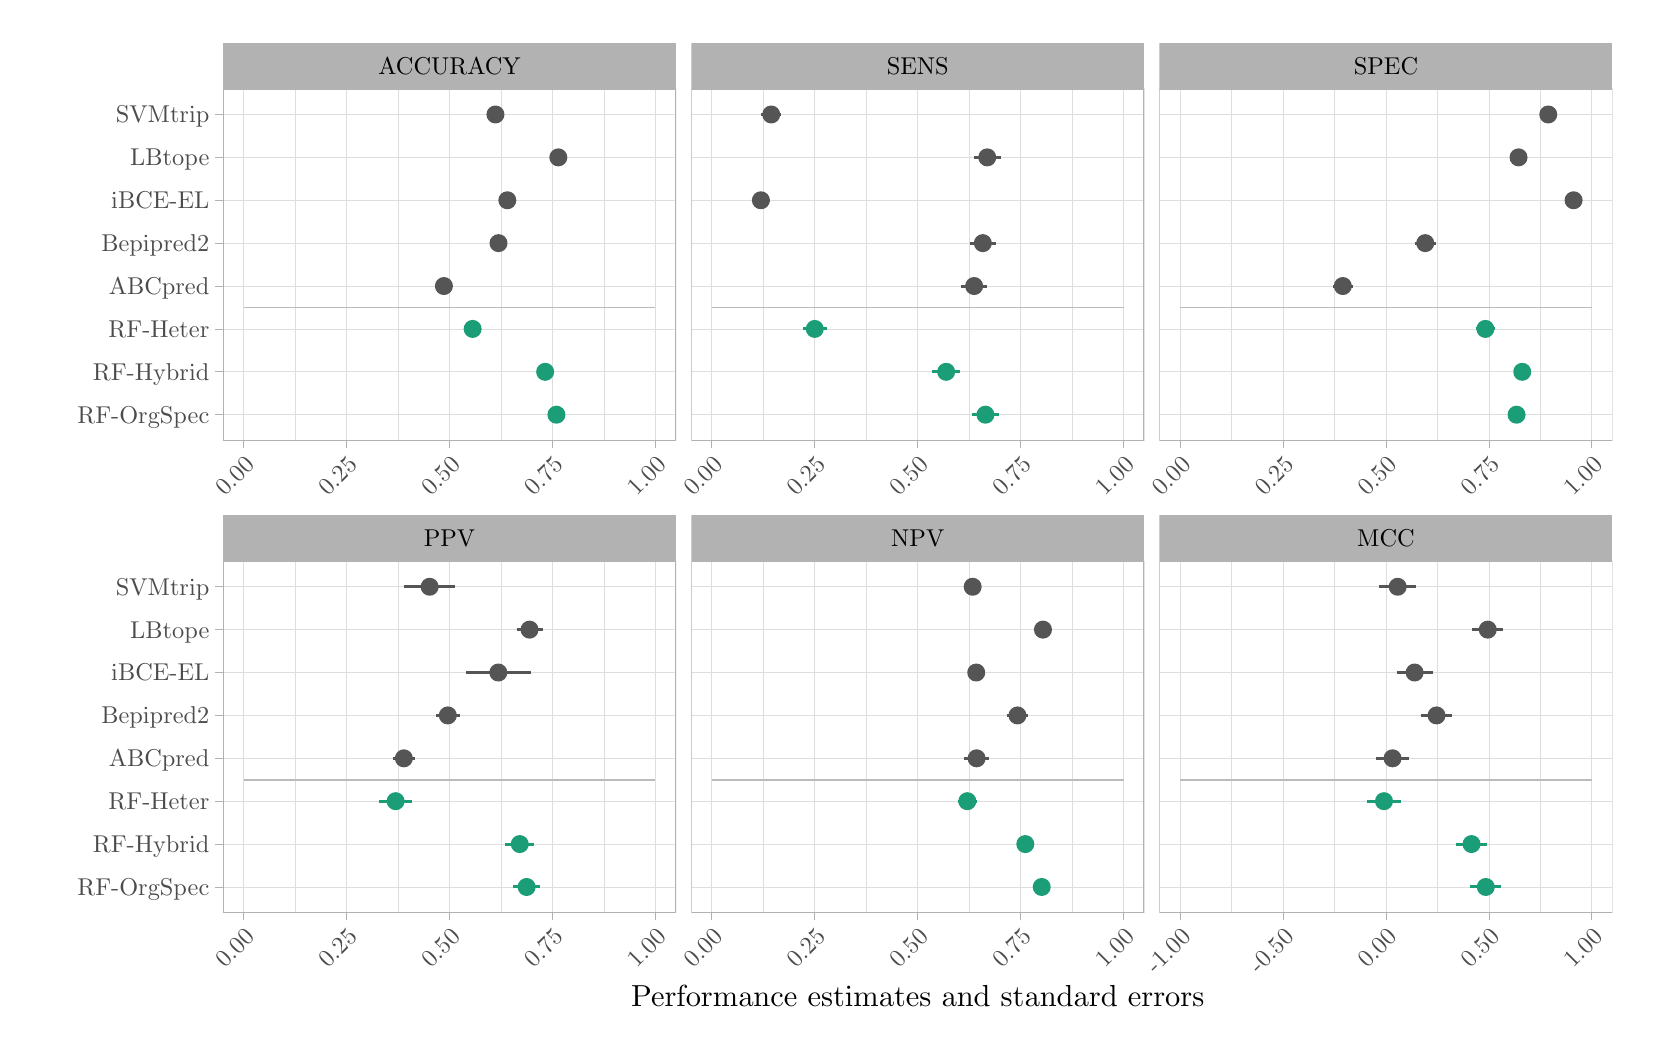
\begin{tikzpicture}[x=1pt,y=1pt]
\definecolor{fillColor}{RGB}{255,255,255}
\path[use as bounding box,fill=fillColor,fill opacity=0.00] (0,0) rectangle (578.16,361.35);
\begin{scope}
\path[clip] (  0.00,  0.00) rectangle (578.16,361.35);
\definecolor{drawColor}{RGB}{255,255,255}
\definecolor{fillColor}{RGB}{255,255,255}

\path[draw=drawColor,line width= 0.6pt,line join=round,line cap=round,fill=fillColor] (  0.00,  0.00) rectangle (578.16,361.35);
\end{scope}
\begin{scope}
\path[clip] ( 70.59,212.20) rectangle (234.28,339.28);
\definecolor{fillColor}{RGB}{255,255,255}

\path[fill=fillColor] ( 70.59,212.20) rectangle (234.28,339.28);
\definecolor{drawColor}{gray}{0.87}

\path[draw=drawColor,line width= 0.1pt,line join=round] ( 96.64,212.20) --
	( 96.64,339.28);

\path[draw=drawColor,line width= 0.1pt,line join=round] (133.84,212.20) --
	(133.84,339.28);

\path[draw=drawColor,line width= 0.1pt,line join=round] (171.04,212.20) --
	(171.04,339.28);

\path[draw=drawColor,line width= 0.1pt,line join=round] (208.24,212.20) --
	(208.24,339.28);

\path[draw=drawColor,line width= 0.3pt,line join=round] ( 70.59,221.50) --
	(234.28,221.50);

\path[draw=drawColor,line width= 0.3pt,line join=round] ( 70.59,236.99) --
	(234.28,236.99);

\path[draw=drawColor,line width= 0.3pt,line join=round] ( 70.59,252.49) --
	(234.28,252.49);

\path[draw=drawColor,line width= 0.3pt,line join=round] ( 70.59,267.99) --
	(234.28,267.99);

\path[draw=drawColor,line width= 0.3pt,line join=round] ( 70.59,283.49) --
	(234.28,283.49);

\path[draw=drawColor,line width= 0.3pt,line join=round] ( 70.59,298.98) --
	(234.28,298.98);

\path[draw=drawColor,line width= 0.3pt,line join=round] ( 70.59,314.48) --
	(234.28,314.48);

\path[draw=drawColor,line width= 0.3pt,line join=round] ( 70.59,329.98) --
	(234.28,329.98);

\path[draw=drawColor,line width= 0.3pt,line join=round] ( 78.03,212.20) --
	( 78.03,339.28);

\path[draw=drawColor,line width= 0.3pt,line join=round] (115.24,212.20) --
	(115.24,339.28);

\path[draw=drawColor,line width= 0.3pt,line join=round] (152.44,212.20) --
	(152.44,339.28);

\path[draw=drawColor,line width= 0.3pt,line join=round] (189.64,212.20) --
	(189.64,339.28);

\path[draw=drawColor,line width= 0.3pt,line join=round] (226.84,212.20) --
	(226.84,339.28);
\definecolor{drawColor}{RGB}{27,158,119}

\path[draw=drawColor,line width= 1.1pt,line join=round] (188.45,221.50) -- (193.68,221.50);

\path[draw=drawColor,line width= 1.1pt,line join=round] (184.34,236.99) -- (189.64,236.99);

\path[draw=drawColor,line width= 1.1pt,line join=round] (157.75,252.49) -- (163.83,252.49);
\definecolor{drawColor}{RGB}{85,85,85}

\path[draw=drawColor,line width= 1.1pt,line join=round] (147.34,267.99) -- (153.47,267.99);

\path[draw=drawColor,line width= 1.1pt,line join=round] (167.24,283.49) -- (173.04,283.49);

\path[draw=drawColor,line width= 1.1pt,line join=round] (170.36,298.98) -- (176.27,298.98);

\path[draw=drawColor,line width= 1.1pt,line join=round] (189.07,314.48) -- (194.43,314.48);

\path[draw=drawColor,line width= 1.1pt,line join=round] (165.97,329.98) -- (172.08,329.98);
\definecolor{drawColor}{RGB}{27,158,119}
\definecolor{fillColor}{RGB}{27,158,119}

\path[draw=drawColor,line width= 0.8pt,line join=round,line cap=round,fill=fillColor] (191.06,221.50) circle (  2.85);

\path[draw=drawColor,line width= 0.8pt,line join=round,line cap=round,fill=fillColor] (186.99,236.99) circle (  2.85);

\path[draw=drawColor,line width= 0.8pt,line join=round,line cap=round,fill=fillColor] (160.79,252.49) circle (  2.85);
\definecolor{drawColor}{RGB}{85,85,85}
\definecolor{fillColor}{RGB}{85,85,85}

\path[draw=drawColor,line width= 0.8pt,line join=round,line cap=round,fill=fillColor] (150.41,267.99) circle (  2.85);

\path[draw=drawColor,line width= 0.8pt,line join=round,line cap=round,fill=fillColor] (170.14,283.49) circle (  2.85);

\path[draw=drawColor,line width= 0.8pt,line join=round,line cap=round,fill=fillColor] (173.32,298.98) circle (  2.85);

\path[draw=drawColor,line width= 0.8pt,line join=round,line cap=round,fill=fillColor] (191.75,314.48) circle (  2.85);

\path[draw=drawColor,line width= 0.8pt,line join=round,line cap=round,fill=fillColor] (169.03,329.98) circle (  2.85);
\definecolor{drawColor}{RGB}{187,187,187}

\path[draw=drawColor,line width= 0.6pt,line join=round] ( 78.03,260.24) -- (226.84,260.24);
\definecolor{drawColor}{gray}{0.70}

\path[draw=drawColor,line width= 0.6pt,line join=round,line cap=round] ( 70.59,212.20) rectangle (234.28,339.28);
\end{scope}
\begin{scope}
\path[clip] ( 70.59, 41.54) rectangle (234.28,168.62);
\definecolor{fillColor}{RGB}{255,255,255}

\path[fill=fillColor] ( 70.59, 41.54) rectangle (234.28,168.62);
\definecolor{drawColor}{gray}{0.87}

\path[draw=drawColor,line width= 0.1pt,line join=round] ( 96.64, 41.54) --
	( 96.64,168.62);

\path[draw=drawColor,line width= 0.1pt,line join=round] (133.84, 41.54) --
	(133.84,168.62);

\path[draw=drawColor,line width= 0.1pt,line join=round] (171.04, 41.54) --
	(171.04,168.62);

\path[draw=drawColor,line width= 0.1pt,line join=round] (208.24, 41.54) --
	(208.24,168.62);

\path[draw=drawColor,line width= 0.3pt,line join=round] ( 70.59, 50.84) --
	(234.28, 50.84);

\path[draw=drawColor,line width= 0.3pt,line join=round] ( 70.59, 66.34) --
	(234.28, 66.34);

\path[draw=drawColor,line width= 0.3pt,line join=round] ( 70.59, 81.84) --
	(234.28, 81.84);

\path[draw=drawColor,line width= 0.3pt,line join=round] ( 70.59, 97.33) --
	(234.28, 97.33);

\path[draw=drawColor,line width= 0.3pt,line join=round] ( 70.59,112.83) --
	(234.28,112.83);

\path[draw=drawColor,line width= 0.3pt,line join=round] ( 70.59,128.33) --
	(234.28,128.33);

\path[draw=drawColor,line width= 0.3pt,line join=round] ( 70.59,143.83) --
	(234.28,143.83);

\path[draw=drawColor,line width= 0.3pt,line join=round] ( 70.59,159.32) --
	(234.28,159.32);

\path[draw=drawColor,line width= 0.3pt,line join=round] ( 78.03, 41.54) --
	( 78.03,168.62);

\path[draw=drawColor,line width= 0.3pt,line join=round] (115.24, 41.54) --
	(115.24,168.62);

\path[draw=drawColor,line width= 0.3pt,line join=round] (152.44, 41.54) --
	(152.44,168.62);

\path[draw=drawColor,line width= 0.3pt,line join=round] (189.64, 41.54) --
	(189.64,168.62);

\path[draw=drawColor,line width= 0.3pt,line join=round] (226.84, 41.54) --
	(226.84,168.62);
\definecolor{drawColor}{RGB}{27,158,119}

\path[draw=drawColor,line width= 1.1pt,line join=round] (175.50, 50.84) -- (185.10, 50.84);

\path[draw=drawColor,line width= 1.1pt,line join=round] (172.60, 66.34) -- (183.05, 66.34);

\path[draw=drawColor,line width= 1.1pt,line join=round] (126.98, 81.84) -- (138.93, 81.84);
\definecolor{drawColor}{RGB}{85,85,85}

\path[draw=drawColor,line width= 1.1pt,line join=round] (132.00, 97.33) -- (139.89, 97.33);

\path[draw=drawColor,line width= 1.1pt,line join=round] (147.57,112.83) -- (156.07,112.83);

\path[draw=drawColor,line width= 1.1pt,line join=round] (158.37,128.33) -- (181.77,128.33);

\path[draw=drawColor,line width= 1.1pt,line join=round] (176.65,143.83) -- (186.06,143.83);

\path[draw=drawColor,line width= 1.1pt,line join=round] (135.97,159.32) -- (154.53,159.32);
\definecolor{drawColor}{RGB}{27,158,119}
\definecolor{fillColor}{RGB}{27,158,119}

\path[draw=drawColor,line width= 0.8pt,line join=round,line cap=round,fill=fillColor] (180.30, 50.84) circle (  2.85);

\path[draw=drawColor,line width= 0.8pt,line join=round,line cap=round,fill=fillColor] (177.82, 66.34) circle (  2.85);

\path[draw=drawColor,line width= 0.8pt,line join=round,line cap=round,fill=fillColor] (132.96, 81.84) circle (  2.85);
\definecolor{drawColor}{RGB}{85,85,85}
\definecolor{fillColor}{RGB}{85,85,85}

\path[draw=drawColor,line width= 0.8pt,line join=round,line cap=round,fill=fillColor] (135.94, 97.33) circle (  2.85);

\path[draw=drawColor,line width= 0.8pt,line join=round,line cap=round,fill=fillColor] (151.82,112.83) circle (  2.85);

\path[draw=drawColor,line width= 0.8pt,line join=round,line cap=round,fill=fillColor] (170.07,128.33) circle (  2.85);

\path[draw=drawColor,line width= 0.8pt,line join=round,line cap=round,fill=fillColor] (181.35,143.83) circle (  2.85);

\path[draw=drawColor,line width= 0.8pt,line join=round,line cap=round,fill=fillColor] (145.25,159.32) circle (  2.85);
\definecolor{drawColor}{RGB}{187,187,187}

\path[draw=drawColor,line width= 0.6pt,line join=round] ( 78.03, 89.59) -- (226.84, 89.59);
\definecolor{drawColor}{gray}{0.70}

\path[draw=drawColor,line width= 0.6pt,line join=round,line cap=round] ( 70.59, 41.54) rectangle (234.28,168.62);
\end{scope}
\begin{scope}
\path[clip] (239.78,212.20) rectangle (403.47,339.28);
\definecolor{fillColor}{RGB}{255,255,255}

\path[fill=fillColor] (239.78,212.20) rectangle (403.47,339.28);
\definecolor{drawColor}{gray}{0.87}

\path[draw=drawColor,line width= 0.1pt,line join=round] (265.82,212.20) --
	(265.82,339.28);

\path[draw=drawColor,line width= 0.1pt,line join=round] (303.03,212.20) --
	(303.03,339.28);

\path[draw=drawColor,line width= 0.1pt,line join=round] (340.23,212.20) --
	(340.23,339.28);

\path[draw=drawColor,line width= 0.1pt,line join=round] (377.43,212.20) --
	(377.43,339.28);

\path[draw=drawColor,line width= 0.3pt,line join=round] (239.78,221.50) --
	(403.47,221.50);

\path[draw=drawColor,line width= 0.3pt,line join=round] (239.78,236.99) --
	(403.47,236.99);

\path[draw=drawColor,line width= 0.3pt,line join=round] (239.78,252.49) --
	(403.47,252.49);

\path[draw=drawColor,line width= 0.3pt,line join=round] (239.78,267.99) --
	(403.47,267.99);

\path[draw=drawColor,line width= 0.3pt,line join=round] (239.78,283.49) --
	(403.47,283.49);

\path[draw=drawColor,line width= 0.3pt,line join=round] (239.78,298.98) --
	(403.47,298.98);

\path[draw=drawColor,line width= 0.3pt,line join=round] (239.78,314.48) --
	(403.47,314.48);

\path[draw=drawColor,line width= 0.3pt,line join=round] (239.78,329.98) --
	(403.47,329.98);

\path[draw=drawColor,line width= 0.3pt,line join=round] (247.22,212.20) --
	(247.22,339.28);

\path[draw=drawColor,line width= 0.3pt,line join=round] (284.43,212.20) --
	(284.43,339.28);

\path[draw=drawColor,line width= 0.3pt,line join=round] (321.63,212.20) --
	(321.63,339.28);

\path[draw=drawColor,line width= 0.3pt,line join=round] (358.83,212.20) --
	(358.83,339.28);

\path[draw=drawColor,line width= 0.3pt,line join=round] (396.03,212.20) --
	(396.03,339.28);
\definecolor{drawColor}{RGB}{27,158,119}

\path[draw=drawColor,line width= 1.1pt,line join=round] (341.33,221.50) -- (350.85,221.50);

\path[draw=drawColor,line width= 1.1pt,line join=round] (326.95,236.99) -- (336.83,236.99);

\path[draw=drawColor,line width= 1.1pt,line join=round] (280.12,252.49) -- (288.72,252.49);
\definecolor{drawColor}{RGB}{85,85,85}

\path[draw=drawColor,line width= 1.1pt,line join=round] (337.19,267.99) -- (346.80,267.99);

\path[draw=drawColor,line width= 1.1pt,line join=round] (340.41,283.49) -- (349.89,283.49);

\path[draw=drawColor,line width= 1.1pt,line join=round] (261.59,298.98) -- (268.30,298.98);

\path[draw=drawColor,line width= 1.1pt,line join=round] (341.88,314.48) -- (351.61,314.48);

\path[draw=drawColor,line width= 1.1pt,line join=round] (265.14,329.98) -- (272.21,329.98);
\definecolor{drawColor}{RGB}{27,158,119}
\definecolor{fillColor}{RGB}{27,158,119}

\path[draw=drawColor,line width= 0.8pt,line join=round,line cap=round,fill=fillColor] (346.09,221.50) circle (  2.85);

\path[draw=drawColor,line width= 0.8pt,line join=round,line cap=round,fill=fillColor] (331.89,236.99) circle (  2.85);

\path[draw=drawColor,line width= 0.8pt,line join=round,line cap=round,fill=fillColor] (284.42,252.49) circle (  2.85);
\definecolor{drawColor}{RGB}{85,85,85}
\definecolor{fillColor}{RGB}{85,85,85}

\path[draw=drawColor,line width= 0.8pt,line join=round,line cap=round,fill=fillColor] (342.00,267.99) circle (  2.85);

\path[draw=drawColor,line width= 0.8pt,line join=round,line cap=round,fill=fillColor] (345.15,283.49) circle (  2.85);

\path[draw=drawColor,line width= 0.8pt,line join=round,line cap=round,fill=fillColor] (264.95,298.98) circle (  2.85);

\path[draw=drawColor,line width= 0.8pt,line join=round,line cap=round,fill=fillColor] (346.74,314.48) circle (  2.85);

\path[draw=drawColor,line width= 0.8pt,line join=round,line cap=round,fill=fillColor] (268.68,329.98) circle (  2.85);
\definecolor{drawColor}{RGB}{187,187,187}

\path[draw=drawColor,line width= 0.6pt,line join=round] (247.22,260.24) -- (396.03,260.24);
\definecolor{drawColor}{gray}{0.70}

\path[draw=drawColor,line width= 0.6pt,line join=round,line cap=round] (239.78,212.20) rectangle (403.47,339.28);
\end{scope}
\begin{scope}
\path[clip] (239.78, 41.54) rectangle (403.47,168.62);
\definecolor{fillColor}{RGB}{255,255,255}

\path[fill=fillColor] (239.78, 41.54) rectangle (403.47,168.62);
\definecolor{drawColor}{gray}{0.87}

\path[draw=drawColor,line width= 0.1pt,line join=round] (265.82, 41.54) --
	(265.82,168.62);

\path[draw=drawColor,line width= 0.1pt,line join=round] (303.03, 41.54) --
	(303.03,168.62);

\path[draw=drawColor,line width= 0.1pt,line join=round] (340.23, 41.54) --
	(340.23,168.62);

\path[draw=drawColor,line width= 0.1pt,line join=round] (377.43, 41.54) --
	(377.43,168.62);

\path[draw=drawColor,line width= 0.3pt,line join=round] (239.78, 50.84) --
	(403.47, 50.84);

\path[draw=drawColor,line width= 0.3pt,line join=round] (239.78, 66.34) --
	(403.47, 66.34);

\path[draw=drawColor,line width= 0.3pt,line join=round] (239.78, 81.84) --
	(403.47, 81.84);

\path[draw=drawColor,line width= 0.3pt,line join=round] (239.78, 97.33) --
	(403.47, 97.33);

\path[draw=drawColor,line width= 0.3pt,line join=round] (239.78,112.83) --
	(403.47,112.83);

\path[draw=drawColor,line width= 0.3pt,line join=round] (239.78,128.33) --
	(403.47,128.33);

\path[draw=drawColor,line width= 0.3pt,line join=round] (239.78,143.83) --
	(403.47,143.83);

\path[draw=drawColor,line width= 0.3pt,line join=round] (239.78,159.32) --
	(403.47,159.32);

\path[draw=drawColor,line width= 0.3pt,line join=round] (247.22, 41.54) --
	(247.22,168.62);

\path[draw=drawColor,line width= 0.3pt,line join=round] (284.43, 41.54) --
	(284.43,168.62);

\path[draw=drawColor,line width= 0.3pt,line join=round] (321.63, 41.54) --
	(321.63,168.62);

\path[draw=drawColor,line width= 0.3pt,line join=round] (358.83, 41.54) --
	(358.83,168.62);

\path[draw=drawColor,line width= 0.3pt,line join=round] (396.03, 41.54) --
	(396.03,168.62);
\definecolor{drawColor}{RGB}{27,158,119}

\path[draw=drawColor,line width= 1.1pt,line join=round] (363.40, 50.84) -- (369.45, 50.84);

\path[draw=drawColor,line width= 1.1pt,line join=round] (357.40, 66.34) -- (363.59, 66.34);

\path[draw=drawColor,line width= 1.1pt,line join=round] (336.11, 81.84) -- (342.97, 81.84);
\definecolor{drawColor}{RGB}{85,85,85}

\path[draw=drawColor,line width= 1.1pt,line join=round] (338.30, 97.33) -- (347.48, 97.33);

\path[draw=drawColor,line width= 1.1pt,line join=round] (353.84,112.83) -- (361.48,112.83);

\path[draw=drawColor,line width= 1.1pt,line join=round] (339.68,128.33) -- (345.84,128.33);

\path[draw=drawColor,line width= 1.1pt,line join=round] (363.73,143.83) -- (370.00,143.83);

\path[draw=drawColor,line width= 1.1pt,line join=round] (338.29,159.32) -- (344.65,159.32);
\definecolor{drawColor}{RGB}{27,158,119}
\definecolor{fillColor}{RGB}{27,158,119}

\path[draw=drawColor,line width= 0.8pt,line join=round,line cap=round,fill=fillColor] (366.42, 50.84) circle (  2.85);

\path[draw=drawColor,line width= 0.8pt,line join=round,line cap=round,fill=fillColor] (360.49, 66.34) circle (  2.85);

\path[draw=drawColor,line width= 0.8pt,line join=round,line cap=round,fill=fillColor] (339.54, 81.84) circle (  2.85);
\definecolor{drawColor}{RGB}{85,85,85}
\definecolor{fillColor}{RGB}{85,85,85}

\path[draw=drawColor,line width= 0.8pt,line join=round,line cap=round,fill=fillColor] (342.89, 97.33) circle (  2.85);

\path[draw=drawColor,line width= 0.8pt,line join=round,line cap=round,fill=fillColor] (357.66,112.83) circle (  2.85);

\path[draw=drawColor,line width= 0.8pt,line join=round,line cap=round,fill=fillColor] (342.76,128.33) circle (  2.85);

\path[draw=drawColor,line width= 0.8pt,line join=round,line cap=round,fill=fillColor] (366.87,143.83) circle (  2.85);

\path[draw=drawColor,line width= 0.8pt,line join=round,line cap=round,fill=fillColor] (341.47,159.32) circle (  2.85);
\definecolor{drawColor}{RGB}{187,187,187}

\path[draw=drawColor,line width= 0.6pt,line join=round] (247.22, 89.59) -- (396.03, 89.59);
\definecolor{drawColor}{gray}{0.70}

\path[draw=drawColor,line width= 0.6pt,line join=round,line cap=round] (239.78, 41.54) rectangle (403.47,168.62);
\end{scope}
\begin{scope}
\path[clip] (408.97,212.20) rectangle (572.66,339.28);
\definecolor{fillColor}{RGB}{255,255,255}

\path[fill=fillColor] (408.97,212.20) rectangle (572.66,339.28);
\definecolor{drawColor}{gray}{0.87}

\path[draw=drawColor,line width= 0.1pt,line join=round] (435.01,212.20) --
	(435.01,339.28);

\path[draw=drawColor,line width= 0.1pt,line join=round] (472.21,212.20) --
	(472.21,339.28);

\path[draw=drawColor,line width= 0.1pt,line join=round] (509.42,212.20) --
	(509.42,339.28);

\path[draw=drawColor,line width= 0.1pt,line join=round] (546.62,212.20) --
	(546.62,339.28);

\path[draw=drawColor,line width= 0.3pt,line join=round] (408.97,221.50) --
	(572.66,221.50);

\path[draw=drawColor,line width= 0.3pt,line join=round] (408.97,236.99) --
	(572.66,236.99);

\path[draw=drawColor,line width= 0.3pt,line join=round] (408.97,252.49) --
	(572.66,252.49);

\path[draw=drawColor,line width= 0.3pt,line join=round] (408.97,267.99) --
	(572.66,267.99);

\path[draw=drawColor,line width= 0.3pt,line join=round] (408.97,283.49) --
	(572.66,283.49);

\path[draw=drawColor,line width= 0.3pt,line join=round] (408.97,298.98) --
	(572.66,298.98);

\path[draw=drawColor,line width= 0.3pt,line join=round] (408.97,314.48) --
	(572.66,314.48);

\path[draw=drawColor,line width= 0.3pt,line join=round] (408.97,329.98) --
	(572.66,329.98);

\path[draw=drawColor,line width= 0.3pt,line join=round] (416.41,212.20) --
	(416.41,339.28);

\path[draw=drawColor,line width= 0.3pt,line join=round] (453.61,212.20) --
	(453.61,339.28);

\path[draw=drawColor,line width= 0.3pt,line join=round] (490.82,212.20) --
	(490.82,339.28);

\path[draw=drawColor,line width= 0.3pt,line join=round] (528.02,212.20) --
	(528.02,339.28);

\path[draw=drawColor,line width= 0.3pt,line join=round] (565.22,212.20) --
	(565.22,339.28);
\definecolor{drawColor}{RGB}{27,158,119}

\path[draw=drawColor,line width= 1.1pt,line join=round] (534.98,221.50) -- (541.03,221.50);

\path[draw=drawColor,line width= 1.1pt,line join=round] (537.05,236.99) -- (543.06,236.99);

\path[draw=drawColor,line width= 1.1pt,line join=round] (523.18,252.49) -- (530.28,252.49);
\definecolor{drawColor}{RGB}{85,85,85}

\path[draw=drawColor,line width= 1.1pt,line join=round] (471.52,267.99) -- (478.95,267.99);

\path[draw=drawColor,line width= 1.1pt,line join=round] (501.15,283.49) -- (508.84,283.49);

\path[draw=drawColor,line width= 1.1pt,line join=round] (556.97,298.98) -- (560.26,298.98);

\path[draw=drawColor,line width= 1.1pt,line join=round] (535.73,314.48) -- (541.71,314.48);

\path[draw=drawColor,line width= 1.1pt,line join=round] (547.02,329.98) -- (551.90,329.98);
\definecolor{drawColor}{RGB}{27,158,119}
\definecolor{fillColor}{RGB}{27,158,119}

\path[draw=drawColor,line width= 0.8pt,line join=round,line cap=round,fill=fillColor] (538.00,221.50) circle (  2.85);

\path[draw=drawColor,line width= 0.8pt,line join=round,line cap=round,fill=fillColor] (540.05,236.99) circle (  2.85);

\path[draw=drawColor,line width= 0.8pt,line join=round,line cap=round,fill=fillColor] (526.73,252.49) circle (  2.85);
\definecolor{drawColor}{RGB}{85,85,85}
\definecolor{fillColor}{RGB}{85,85,85}

\path[draw=drawColor,line width= 0.8pt,line join=round,line cap=round,fill=fillColor] (475.23,267.99) circle (  2.85);

\path[draw=drawColor,line width= 0.8pt,line join=round,line cap=round,fill=fillColor] (505.00,283.49) circle (  2.85);

\path[draw=drawColor,line width= 0.8pt,line join=round,line cap=round,fill=fillColor] (558.61,298.98) circle (  2.85);

\path[draw=drawColor,line width= 0.8pt,line join=round,line cap=round,fill=fillColor] (538.72,314.48) circle (  2.85);

\path[draw=drawColor,line width= 0.8pt,line join=round,line cap=round,fill=fillColor] (549.46,329.98) circle (  2.85);
\definecolor{drawColor}{RGB}{187,187,187}

\path[draw=drawColor,line width= 0.6pt,line join=round] (416.41,260.24) -- (565.22,260.24);
\definecolor{drawColor}{gray}{0.70}

\path[draw=drawColor,line width= 0.6pt,line join=round,line cap=round] (408.97,212.20) rectangle (572.66,339.28);
\end{scope}
\begin{scope}
\path[clip] (408.97, 41.54) rectangle (572.66,168.62);
\definecolor{fillColor}{RGB}{255,255,255}

\path[fill=fillColor] (408.97, 41.54) rectangle (572.66,168.62);
\definecolor{drawColor}{gray}{0.87}

\path[draw=drawColor,line width= 0.1pt,line join=round] (435.01, 41.54) --
	(435.01,168.62);

\path[draw=drawColor,line width= 0.1pt,line join=round] (472.21, 41.54) --
	(472.21,168.62);

\path[draw=drawColor,line width= 0.1pt,line join=round] (509.42, 41.54) --
	(509.42,168.62);

\path[draw=drawColor,line width= 0.1pt,line join=round] (546.62, 41.54) --
	(546.62,168.62);

\path[draw=drawColor,line width= 0.3pt,line join=round] (408.97, 50.84) --
	(572.66, 50.84);

\path[draw=drawColor,line width= 0.3pt,line join=round] (408.97, 66.34) --
	(572.66, 66.34);

\path[draw=drawColor,line width= 0.3pt,line join=round] (408.97, 81.84) --
	(572.66, 81.84);

\path[draw=drawColor,line width= 0.3pt,line join=round] (408.97, 97.33) --
	(572.66, 97.33);

\path[draw=drawColor,line width= 0.3pt,line join=round] (408.97,112.83) --
	(572.66,112.83);

\path[draw=drawColor,line width= 0.3pt,line join=round] (408.97,128.33) --
	(572.66,128.33);

\path[draw=drawColor,line width= 0.3pt,line join=round] (408.97,143.83) --
	(572.66,143.83);

\path[draw=drawColor,line width= 0.3pt,line join=round] (408.97,159.32) --
	(572.66,159.32);

\path[draw=drawColor,line width= 0.3pt,line join=round] (416.41, 41.54) --
	(416.41,168.62);

\path[draw=drawColor,line width= 0.3pt,line join=round] (453.61, 41.54) --
	(453.61,168.62);

\path[draw=drawColor,line width= 0.3pt,line join=round] (490.82, 41.54) --
	(490.82,168.62);

\path[draw=drawColor,line width= 0.3pt,line join=round] (528.02, 41.54) --
	(528.02,168.62);

\path[draw=drawColor,line width= 0.3pt,line join=round] (565.22, 41.54) --
	(565.22,168.62);
\definecolor{drawColor}{RGB}{27,158,119}

\path[draw=drawColor,line width= 1.1pt,line join=round] (521.29, 50.84) -- (532.48, 50.84);

\path[draw=drawColor,line width= 1.1pt,line join=round] (516.02, 66.34) -- (527.44, 66.34);

\path[draw=drawColor,line width= 1.1pt,line join=round] (483.96, 81.84) -- (496.25, 81.84);
\definecolor{drawColor}{RGB}{85,85,85}

\path[draw=drawColor,line width= 1.1pt,line join=round] (487.15, 97.33) -- (499.26, 97.33);

\path[draw=drawColor,line width= 1.1pt,line join=round] (503.34,112.83) -- (514.83,112.83);

\path[draw=drawColor,line width= 1.1pt,line join=round] (494.63,128.33) -- (507.71,128.33);

\path[draw=drawColor,line width= 1.1pt,line join=round] (521.93,143.83) -- (533.28,143.83);

\path[draw=drawColor,line width= 1.1pt,line join=round] (488.47,159.32) -- (501.64,159.32);
\definecolor{drawColor}{RGB}{27,158,119}
\definecolor{fillColor}{RGB}{27,158,119}

\path[draw=drawColor,line width= 0.8pt,line join=round,line cap=round,fill=fillColor] (526.89, 50.84) circle (  2.85);

\path[draw=drawColor,line width= 0.8pt,line join=round,line cap=round,fill=fillColor] (521.73, 66.34) circle (  2.85);

\path[draw=drawColor,line width= 0.8pt,line join=round,line cap=round,fill=fillColor] (490.10, 81.84) circle (  2.85);
\definecolor{drawColor}{RGB}{85,85,85}
\definecolor{fillColor}{RGB}{85,85,85}

\path[draw=drawColor,line width= 0.8pt,line join=round,line cap=round,fill=fillColor] (493.20, 97.33) circle (  2.85);

\path[draw=drawColor,line width= 0.8pt,line join=round,line cap=round,fill=fillColor] (509.09,112.83) circle (  2.85);

\path[draw=drawColor,line width= 0.8pt,line join=round,line cap=round,fill=fillColor] (501.17,128.33) circle (  2.85);

\path[draw=drawColor,line width= 0.8pt,line join=round,line cap=round,fill=fillColor] (527.60,143.83) circle (  2.85);

\path[draw=drawColor,line width= 0.8pt,line join=round,line cap=round,fill=fillColor] (495.05,159.32) circle (  2.85);
\definecolor{drawColor}{RGB}{187,187,187}

\path[draw=drawColor,line width= 0.6pt,line join=round] (416.41, 89.59) -- (565.22, 89.59);
\definecolor{drawColor}{gray}{0.70}

\path[draw=drawColor,line width= 0.6pt,line join=round,line cap=round] (408.97, 41.54) rectangle (572.66,168.62);
\end{scope}
\begin{scope}
\path[clip] ( 70.59,168.62) rectangle (234.28,185.19);
\definecolor{fillColor}{gray}{0.70}

\path[fill=fillColor] ( 70.59,168.62) rectangle (234.28,185.19);
\definecolor{drawColor}{RGB}{0,0,0}

\node[text=drawColor,anchor=base,inner sep=0pt, outer sep=0pt, scale=  0.88] at (152.44,173.88) {PPV};
\end{scope}
\begin{scope}
\path[clip] (239.78,168.62) rectangle (403.47,185.19);
\definecolor{fillColor}{gray}{0.70}

\path[fill=fillColor] (239.78,168.62) rectangle (403.47,185.19);
\definecolor{drawColor}{RGB}{0,0,0}

\node[text=drawColor,anchor=base,inner sep=0pt, outer sep=0pt, scale=  0.88] at (321.63,173.88) {NPV};
\end{scope}
\begin{scope}
\path[clip] (408.97,168.62) rectangle (572.66,185.19);
\definecolor{fillColor}{gray}{0.70}

\path[fill=fillColor] (408.97,168.62) rectangle (572.66,185.19);
\definecolor{drawColor}{RGB}{0,0,0}

\node[text=drawColor,anchor=base,inner sep=0pt, outer sep=0pt, scale=  0.88] at (490.82,173.88) {MCC};
\end{scope}
\begin{scope}
\path[clip] ( 70.59,339.28) rectangle (234.28,355.85);
\definecolor{fillColor}{gray}{0.70}

\path[fill=fillColor] ( 70.59,339.28) rectangle (234.28,355.85);
\definecolor{drawColor}{RGB}{0,0,0}

\node[text=drawColor,anchor=base,inner sep=0pt, outer sep=0pt, scale=  0.88] at (152.44,344.53) {ACCURACY};
\end{scope}
\begin{scope}
\path[clip] (239.78,339.28) rectangle (403.47,355.85);
\definecolor{fillColor}{gray}{0.70}

\path[fill=fillColor] (239.78,339.28) rectangle (403.47,355.85);
\definecolor{drawColor}{RGB}{0,0,0}

\node[text=drawColor,anchor=base,inner sep=0pt, outer sep=0pt, scale=  0.88] at (321.63,344.53) {SENS};
\end{scope}
\begin{scope}
\path[clip] (408.97,339.28) rectangle (572.66,355.85);
\definecolor{fillColor}{gray}{0.70}

\path[fill=fillColor] (408.97,339.28) rectangle (572.66,355.85);
\definecolor{drawColor}{RGB}{0,0,0}

\node[text=drawColor,anchor=base,inner sep=0pt, outer sep=0pt, scale=  0.88] at (490.82,344.53) {SPEC};
\end{scope}
\begin{scope}
\path[clip] (  0.00,  0.00) rectangle (578.16,361.35);
\definecolor{drawColor}{gray}{0.70}

\path[draw=drawColor,line width= 0.3pt,line join=round] ( 78.03, 38.79) --
	( 78.03, 41.54);

\path[draw=drawColor,line width= 0.3pt,line join=round] (115.24, 38.79) --
	(115.24, 41.54);

\path[draw=drawColor,line width= 0.3pt,line join=round] (152.44, 38.79) --
	(152.44, 41.54);

\path[draw=drawColor,line width= 0.3pt,line join=round] (189.64, 38.79) --
	(189.64, 41.54);

\path[draw=drawColor,line width= 0.3pt,line join=round] (226.84, 38.79) --
	(226.84, 41.54);
\end{scope}
\begin{scope}
\path[clip] (  0.00,  0.00) rectangle (578.16,361.35);
\definecolor{drawColor}{gray}{0.30}

\node[text=drawColor,rotate= 45.00,anchor=base east,inner sep=0pt, outer sep=0pt, scale=  0.88] at ( 82.32, 32.31) {0.00};

\node[text=drawColor,rotate= 45.00,anchor=base east,inner sep=0pt, outer sep=0pt, scale=  0.88] at (119.52, 32.31) {0.25};

\node[text=drawColor,rotate= 45.00,anchor=base east,inner sep=0pt, outer sep=0pt, scale=  0.88] at (156.72, 32.31) {0.50};

\node[text=drawColor,rotate= 45.00,anchor=base east,inner sep=0pt, outer sep=0pt, scale=  0.88] at (193.93, 32.31) {0.75};

\node[text=drawColor,rotate= 45.00,anchor=base east,inner sep=0pt, outer sep=0pt, scale=  0.88] at (231.13, 32.31) {1.00};
\end{scope}
\begin{scope}
\path[clip] (  0.00,  0.00) rectangle (578.16,361.35);
\definecolor{drawColor}{gray}{0.70}

\path[draw=drawColor,line width= 0.3pt,line join=round] (247.22, 38.79) --
	(247.22, 41.54);

\path[draw=drawColor,line width= 0.3pt,line join=round] (284.43, 38.79) --
	(284.43, 41.54);

\path[draw=drawColor,line width= 0.3pt,line join=round] (321.63, 38.79) --
	(321.63, 41.54);

\path[draw=drawColor,line width= 0.3pt,line join=round] (358.83, 38.79) --
	(358.83, 41.54);

\path[draw=drawColor,line width= 0.3pt,line join=round] (396.03, 38.79) --
	(396.03, 41.54);
\end{scope}
\begin{scope}
\path[clip] (  0.00,  0.00) rectangle (578.16,361.35);
\definecolor{drawColor}{gray}{0.30}

\node[text=drawColor,rotate= 45.00,anchor=base east,inner sep=0pt, outer sep=0pt, scale=  0.88] at (251.51, 32.31) {0.00};

\node[text=drawColor,rotate= 45.00,anchor=base east,inner sep=0pt, outer sep=0pt, scale=  0.88] at (288.71, 32.31) {0.25};

\node[text=drawColor,rotate= 45.00,anchor=base east,inner sep=0pt, outer sep=0pt, scale=  0.88] at (325.91, 32.31) {0.50};

\node[text=drawColor,rotate= 45.00,anchor=base east,inner sep=0pt, outer sep=0pt, scale=  0.88] at (363.11, 32.31) {0.75};

\node[text=drawColor,rotate= 45.00,anchor=base east,inner sep=0pt, outer sep=0pt, scale=  0.88] at (400.32, 32.31) {1.00};
\end{scope}
\begin{scope}
\path[clip] (  0.00,  0.00) rectangle (578.16,361.35);
\definecolor{drawColor}{gray}{0.70}

\path[draw=drawColor,line width= 0.3pt,line join=round] (416.41, 38.79) --
	(416.41, 41.54);

\path[draw=drawColor,line width= 0.3pt,line join=round] (453.61, 38.79) --
	(453.61, 41.54);

\path[draw=drawColor,line width= 0.3pt,line join=round] (490.82, 38.79) --
	(490.82, 41.54);

\path[draw=drawColor,line width= 0.3pt,line join=round] (528.02, 38.79) --
	(528.02, 41.54);

\path[draw=drawColor,line width= 0.3pt,line join=round] (565.22, 38.79) --
	(565.22, 41.54);
\end{scope}
\begin{scope}
\path[clip] (  0.00,  0.00) rectangle (578.16,361.35);
\definecolor{drawColor}{gray}{0.30}

\node[text=drawColor,rotate= 45.00,anchor=base east,inner sep=0pt, outer sep=0pt, scale=  0.88] at (420.70, 32.31) {-1.00};

\node[text=drawColor,rotate= 45.00,anchor=base east,inner sep=0pt, outer sep=0pt, scale=  0.88] at (457.90, 32.31) {-0.50};

\node[text=drawColor,rotate= 45.00,anchor=base east,inner sep=0pt, outer sep=0pt, scale=  0.88] at (495.10, 32.31) {0.00};

\node[text=drawColor,rotate= 45.00,anchor=base east,inner sep=0pt, outer sep=0pt, scale=  0.88] at (532.30, 32.31) {0.50};

\node[text=drawColor,rotate= 45.00,anchor=base east,inner sep=0pt, outer sep=0pt, scale=  0.88] at (569.51, 32.31) {1.00};
\end{scope}
\begin{scope}
\path[clip] (  0.00,  0.00) rectangle (578.16,361.35);
\definecolor{drawColor}{gray}{0.70}

\path[draw=drawColor,line width= 0.3pt,line join=round] ( 78.03,209.45) --
	( 78.03,212.20);

\path[draw=drawColor,line width= 0.3pt,line join=round] (115.24,209.45) --
	(115.24,212.20);

\path[draw=drawColor,line width= 0.3pt,line join=round] (152.44,209.45) --
	(152.44,212.20);

\path[draw=drawColor,line width= 0.3pt,line join=round] (189.64,209.45) --
	(189.64,212.20);

\path[draw=drawColor,line width= 0.3pt,line join=round] (226.84,209.45) --
	(226.84,212.20);
\end{scope}
\begin{scope}
\path[clip] (  0.00,  0.00) rectangle (578.16,361.35);
\definecolor{drawColor}{gray}{0.30}

\node[text=drawColor,rotate= 45.00,anchor=base east,inner sep=0pt, outer sep=0pt, scale=  0.88] at ( 82.32,202.96) {0.00};

\node[text=drawColor,rotate= 45.00,anchor=base east,inner sep=0pt, outer sep=0pt, scale=  0.88] at (119.52,202.96) {0.25};

\node[text=drawColor,rotate= 45.00,anchor=base east,inner sep=0pt, outer sep=0pt, scale=  0.88] at (156.72,202.96) {0.50};

\node[text=drawColor,rotate= 45.00,anchor=base east,inner sep=0pt, outer sep=0pt, scale=  0.88] at (193.93,202.96) {0.75};

\node[text=drawColor,rotate= 45.00,anchor=base east,inner sep=0pt, outer sep=0pt, scale=  0.88] at (231.13,202.96) {1.00};
\end{scope}
\begin{scope}
\path[clip] (  0.00,  0.00) rectangle (578.16,361.35);
\definecolor{drawColor}{gray}{0.70}

\path[draw=drawColor,line width= 0.3pt,line join=round] (247.22,209.45) --
	(247.22,212.20);

\path[draw=drawColor,line width= 0.3pt,line join=round] (284.43,209.45) --
	(284.43,212.20);

\path[draw=drawColor,line width= 0.3pt,line join=round] (321.63,209.45) --
	(321.63,212.20);

\path[draw=drawColor,line width= 0.3pt,line join=round] (358.83,209.45) --
	(358.83,212.20);

\path[draw=drawColor,line width= 0.3pt,line join=round] (396.03,209.45) --
	(396.03,212.20);
\end{scope}
\begin{scope}
\path[clip] (  0.00,  0.00) rectangle (578.16,361.35);
\definecolor{drawColor}{gray}{0.30}

\node[text=drawColor,rotate= 45.00,anchor=base east,inner sep=0pt, outer sep=0pt, scale=  0.88] at (251.51,202.96) {0.00};

\node[text=drawColor,rotate= 45.00,anchor=base east,inner sep=0pt, outer sep=0pt, scale=  0.88] at (288.71,202.96) {0.25};

\node[text=drawColor,rotate= 45.00,anchor=base east,inner sep=0pt, outer sep=0pt, scale=  0.88] at (325.91,202.96) {0.50};

\node[text=drawColor,rotate= 45.00,anchor=base east,inner sep=0pt, outer sep=0pt, scale=  0.88] at (363.11,202.96) {0.75};

\node[text=drawColor,rotate= 45.00,anchor=base east,inner sep=0pt, outer sep=0pt, scale=  0.88] at (400.32,202.96) {1.00};
\end{scope}
\begin{scope}
\path[clip] (  0.00,  0.00) rectangle (578.16,361.35);
\definecolor{drawColor}{gray}{0.70}

\path[draw=drawColor,line width= 0.3pt,line join=round] (416.41,209.45) --
	(416.41,212.20);

\path[draw=drawColor,line width= 0.3pt,line join=round] (453.61,209.45) --
	(453.61,212.20);

\path[draw=drawColor,line width= 0.3pt,line join=round] (490.82,209.45) --
	(490.82,212.20);

\path[draw=drawColor,line width= 0.3pt,line join=round] (528.02,209.45) --
	(528.02,212.20);

\path[draw=drawColor,line width= 0.3pt,line join=round] (565.22,209.45) --
	(565.22,212.20);
\end{scope}
\begin{scope}
\path[clip] (  0.00,  0.00) rectangle (578.16,361.35);
\definecolor{drawColor}{gray}{0.30}

\node[text=drawColor,rotate= 45.00,anchor=base east,inner sep=0pt, outer sep=0pt, scale=  0.88] at (420.70,202.96) {0.00};

\node[text=drawColor,rotate= 45.00,anchor=base east,inner sep=0pt, outer sep=0pt, scale=  0.88] at (457.90,202.96) {0.25};

\node[text=drawColor,rotate= 45.00,anchor=base east,inner sep=0pt, outer sep=0pt, scale=  0.88] at (495.10,202.96) {0.50};

\node[text=drawColor,rotate= 45.00,anchor=base east,inner sep=0pt, outer sep=0pt, scale=  0.88] at (532.30,202.96) {0.75};

\node[text=drawColor,rotate= 45.00,anchor=base east,inner sep=0pt, outer sep=0pt, scale=  0.88] at (569.51,202.96) {1.00};
\end{scope}
\begin{scope}
\path[clip] (  0.00,  0.00) rectangle (578.16,361.35);
\definecolor{drawColor}{gray}{0.30}

\node[text=drawColor,anchor=base east,inner sep=0pt, outer sep=0pt, scale=  0.88] at ( 65.64,218.47) {RF-OrgSpec};

\node[text=drawColor,anchor=base east,inner sep=0pt, outer sep=0pt, scale=  0.88] at ( 65.64,233.96) {RF-Hybrid};

\node[text=drawColor,anchor=base east,inner sep=0pt, outer sep=0pt, scale=  0.88] at ( 65.64,249.46) {RF-Heter};

\node[text=drawColor,anchor=base east,inner sep=0pt, outer sep=0pt, scale=  0.88] at ( 65.64,264.96) {ABCpred};

\node[text=drawColor,anchor=base east,inner sep=0pt, outer sep=0pt, scale=  0.88] at ( 65.64,280.46) {Bepipred2};

\node[text=drawColor,anchor=base east,inner sep=0pt, outer sep=0pt, scale=  0.88] at ( 65.64,295.95) {iBCE-EL};

\node[text=drawColor,anchor=base east,inner sep=0pt, outer sep=0pt, scale=  0.88] at ( 65.64,311.45) {LBtope};

\node[text=drawColor,anchor=base east,inner sep=0pt, outer sep=0pt, scale=  0.88] at ( 65.64,326.95) {SVMtrip};
\end{scope}
\begin{scope}
\path[clip] (  0.00,  0.00) rectangle (578.16,361.35);
\definecolor{drawColor}{gray}{0.70}

\path[draw=drawColor,line width= 0.3pt,line join=round] ( 67.84,221.50) --
	( 70.59,221.50);

\path[draw=drawColor,line width= 0.3pt,line join=round] ( 67.84,236.99) --
	( 70.59,236.99);

\path[draw=drawColor,line width= 0.3pt,line join=round] ( 67.84,252.49) --
	( 70.59,252.49);

\path[draw=drawColor,line width= 0.3pt,line join=round] ( 67.84,267.99) --
	( 70.59,267.99);

\path[draw=drawColor,line width= 0.3pt,line join=round] ( 67.84,283.49) --
	( 70.59,283.49);

\path[draw=drawColor,line width= 0.3pt,line join=round] ( 67.84,298.98) --
	( 70.59,298.98);

\path[draw=drawColor,line width= 0.3pt,line join=round] ( 67.84,314.48) --
	( 70.59,314.48);

\path[draw=drawColor,line width= 0.3pt,line join=round] ( 67.84,329.98) --
	( 70.59,329.98);
\end{scope}
\begin{scope}
\path[clip] (  0.00,  0.00) rectangle (578.16,361.35);
\definecolor{drawColor}{gray}{0.30}

\node[text=drawColor,anchor=base east,inner sep=0pt, outer sep=0pt, scale=  0.88] at ( 65.64, 47.81) {RF-OrgSpec};

\node[text=drawColor,anchor=base east,inner sep=0pt, outer sep=0pt, scale=  0.88] at ( 65.64, 63.31) {RF-Hybrid};

\node[text=drawColor,anchor=base east,inner sep=0pt, outer sep=0pt, scale=  0.88] at ( 65.64, 78.81) {RF-Heter};

\node[text=drawColor,anchor=base east,inner sep=0pt, outer sep=0pt, scale=  0.88] at ( 65.64, 94.30) {ABCpred};

\node[text=drawColor,anchor=base east,inner sep=0pt, outer sep=0pt, scale=  0.88] at ( 65.64,109.80) {Bepipred2};

\node[text=drawColor,anchor=base east,inner sep=0pt, outer sep=0pt, scale=  0.88] at ( 65.64,125.30) {iBCE-EL};

\node[text=drawColor,anchor=base east,inner sep=0pt, outer sep=0pt, scale=  0.88] at ( 65.64,140.80) {LBtope};

\node[text=drawColor,anchor=base east,inner sep=0pt, outer sep=0pt, scale=  0.88] at ( 65.64,156.29) {SVMtrip};
\end{scope}
\begin{scope}
\path[clip] (  0.00,  0.00) rectangle (578.16,361.35);
\definecolor{drawColor}{gray}{0.70}

\path[draw=drawColor,line width= 0.3pt,line join=round] ( 67.84, 50.84) --
	( 70.59, 50.84);

\path[draw=drawColor,line width= 0.3pt,line join=round] ( 67.84, 66.34) --
	( 70.59, 66.34);

\path[draw=drawColor,line width= 0.3pt,line join=round] ( 67.84, 81.84) --
	( 70.59, 81.84);

\path[draw=drawColor,line width= 0.3pt,line join=round] ( 67.84, 97.33) --
	( 70.59, 97.33);

\path[draw=drawColor,line width= 0.3pt,line join=round] ( 67.84,112.83) --
	( 70.59,112.83);

\path[draw=drawColor,line width= 0.3pt,line join=round] ( 67.84,128.33) --
	( 70.59,128.33);

\path[draw=drawColor,line width= 0.3pt,line join=round] ( 67.84,143.83) --
	( 70.59,143.83);

\path[draw=drawColor,line width= 0.3pt,line join=round] ( 67.84,159.32) --
	( 70.59,159.32);
\end{scope}
\begin{scope}
\path[clip] (  0.00,  0.00) rectangle (578.16,361.35);
\definecolor{drawColor}{RGB}{0,0,0}

\node[text=drawColor,anchor=base,inner sep=0pt, outer sep=0pt, scale=  1.10] at (321.63,  7.64) {Performance estimates and standard errors};
\end{scope}
\end{tikzpicture}
